
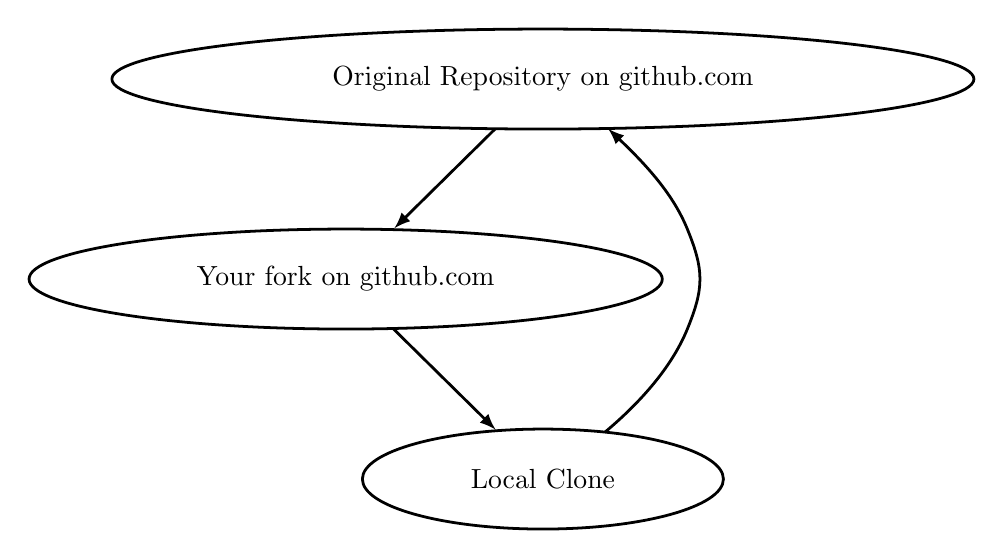
\begin{tikzpicture}[>=latex,line join=bevel,]
  \pgfsetlinewidth{1bp}
%%
\pgfsetcolor{black}
  % Edge: orig -> fork
  \draw [->] (167.55bp,144.05bp) .. controls (158.87bp,135.5bp) and (148.18bp,124.96bp)  .. (131.26bp,108.28bp);
  % Edge: fork -> clone
  \draw [->] (130.93bp,72.055bp) .. controls (139.82bp,63.285bp) and (150.83bp,52.432bp)  .. (167.71bp,35.789bp);
  % Edge: clone -> orig
  \draw [->] (207.14bp,34.94bp) .. controls (218.3bp,44.306bp) and (230.69bp,57.203bp)  .. (236.74bp,72.0bp) .. controls (242.79bp,86.811bp) and (242.79bp,93.189bp)  .. (236.74bp,108.0bp) .. controls (232.21bp,119.08bp) and (224.14bp,129.09bp)  .. (208.22bp,144.14bp);
  % Node: orig
\begin{scope}
  \definecolor{strokecol}{rgb}{0.0,0.0,0.0};
  \pgfsetstrokecolor{strokecol}
  \draw (184.74bp,162.0bp) ellipse (155.17bp and 18.0bp);
  \draw (184.74bp,162.0bp) node {Original Repository on github.com};
\end{scope}
  % Node: fork
\begin{scope}
  \definecolor{strokecol}{rgb}{0.0,0.0,0.0};
  \pgfsetstrokecolor{strokecol}
  \draw (113.74bp,90.0bp) ellipse (113.98bp and 18.0bp);
  \draw (113.74bp,90.0bp) node {Your fork on github.com};
\end{scope}
  % Node: clone
\begin{scope}
  \definecolor{strokecol}{rgb}{0.0,0.0,0.0};
  \pgfsetstrokecolor{strokecol}
  \draw (184.74bp,18.0bp) ellipse (64.99bp and 18.0bp);
  \draw (184.74bp,18.0bp) node {Local Clone};
\end{scope}
%
\end{tikzpicture}

